\chapter{Introduction}
Do not forget to read section~\ref{sec:motivation}. Lorem ipsum dolor sit amet \cite{matlab:ode}, consectetur adipiscing elit. Donec viverra gravida adipiscing \cite{paper:A}. Morbi vitae dui eu leo dapibus venenatis quis laoreet augue. Proin sem nunc, lobortis sed gravida id, iaculis id justo. Sed convallis, mauris vel mattis posuere, tortor quam molestie sem, vel feugiat risus dolor sit amet purus. Nulla facilisi. Duis ac velit non tortor malesuada pellentesque vitae vitae erat. Aliquam dapibus porta lorem lacinia vestibulum. Nulla convallis venenatis euismod. Suspendisse adipiscing lacus id nisi hendrerit dapibus. Sed quam diam, pretium vel accumsan vel, pulvinar et odio. Nulla facilisis ullamcorper metus non suscipit. Aliquam nec augue odio. In hac habitasse platea dictumst. Nulla facilisi. Pellentesque habitant morbi tristique senectus et netus et malesuada fames ac turpis egestas. Maecenas consequat mattis metus, in imperdiet purus suscipit eu. Mauris velit lorem, pharetra nec vehicula cursus, vulputate sit amet dui. Nam sed eros magna, quis molestie urna.
\section{Motivation}\label{sec:motivation}
Just a math thing \( \forall x \in X \) and another one:
\[ \alpha^2 + \beta^2 = \gamma^2 \]

Lorem ipsum dolor sit amet, consectetur adipiscing elit. Donec viverra gravida adipiscing. Morbi vitae dui eu leo dapibus venenatis quis laoreet augue. Proin sem nunc, lobortis sed gravida id, iaculis id justo. Sed convallis, mauris vel mattis posuere, tortor quam molestie sem, vel feugiat risus dolor sit amet purus. Nulla facilisi. Duis ac velit non tortor malesuada pellentesque vitae vitae erat
\begin{table}[h]
  \begin{center}
    \begin{tabular}{| l c r |}
    \hline
    1 & 2 & 3 \\
    4 & 5 & 6 \\
    7 & 8 & 9 \\
    \hline
    \end{tabular}
  \end{center}
  \caption{A simple table}
  \label{tab:simple1}
\end{table}

\autoref{tab:simple1} is a very simple example. Lorem ipsum dolor sit amet, consectetur adipiscing elit. Donec viverra gravida adipiscing. Morbi vitae dui eu leo dapibus venenatis quis laoreet augue. Proin sem nunc, lobortis sed gravida id, iaculis id justo. Sed convallis, mauris vel mattis posuere, tortor quam molestie sem, vel feugiat risus dolor sit amet purus. Nulla facilisi. Duis ac velit non tortor malesuada pellentesque vitae vitae erat. Aliquam dapibus porta lorem lacinia vestibulum. Nulla convallis venenatis euismod. Suspendisse adipiscing lacus id nisi hendrerit dapibus. Sed quam diam, pretium vel accumsan vel, pulvinar et odio. Nulla facilisis ullamcorper metus non suscipit. Aliquam nec augue odio. In hac habitasse platea dictumst. Nulla facilisi. Pellentesque habitant morbi tristique senectus et netus et malesuada fames ac turpis egestas. Maecenas consequat mattis metus, in imperdiet purus suscipit eu. Mauris velit lorem, pharetra nec vehicula cursus, vulputate sit amet dui. Nam sed eros magna, quis molestie urna.
\begin{figure}[h]
    \centering
        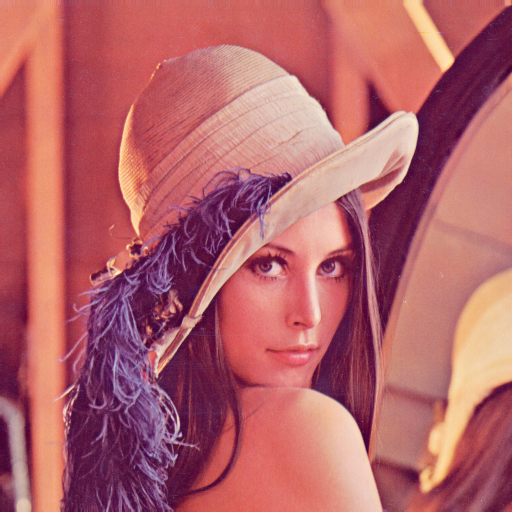
\includegraphics[width=0.8\textwidth]{resources/Lena.png}
    \caption{This is an image}
    \label{fig:lena}
\end{figure}

Figure \ref{fig:lena} shows a picture. Lorem ipsum dolor sit amet, consectetur adipiscing elit. Donec viverra gravida adipiscing. Morbi vitae dui eu leo dapibus venenatis quis laoreet augue. Proin sem nunc, lobortis sed gravida id, iaculis id justo. Sed convallis, mauris vel mattis posuere, tortor quam molestie sem, vel feugiat risus dolor sit amet purus. Nulla facilisi. Duis ac velit non tortor malesuada pellentesque vitae vitae erat. Aliquam dapibus porta lorem lacinia vestibulum. Nulla convallis venenatis euismod. Suspendisse adipiscing lacus id nisi hendrerit dapibus. Sed quam diam, pretium vel accumsan vel, pulvinar et odio. Nulla facilisis ullamcorper metus non suscipit. Aliquam nec augue odio. In hac habitasse platea dictumst. Nulla facilisi. Pellentesque habitant morbi tristique senectus et netus et malesuada fames ac turpis egestas. Maecenas consequat mattis metus, in imperdiet purus suscipit eu. Mauris velit lorem, pharetra nec vehicula cursus, vulputate sit amet dui. Nam sed eros magna, quis molestie urna.
\begin{minted}[]{haskell}
f 0 = 0
f 1 = 1
f a = f (a-1) + f (a-1)
\end{minted}
